% This is a template for your written document.
%
% To compile using latexmk on the command line, run the following: 
% latexmk -pdf main.tex

\documentclass[12pt]{article}
\usepackage{setspace}
\usepackage{graphicx} % used for includegraphics
\singlespace
\usepackage[left=1in,right=1in,top=1in,bottom=1in]{geometry}

\title{\textbf{A Software-Based Comparative Study of Error Sensitivity in Classical and Quantum Optimization Algorithms}}
\author{Aayush Rajak}

\begin{document}

\maketitle

Classical computing processes information using bits that take definite values of 0 or 1, whereas quantum computing uses qubits that can exist in superpositions of states and become entangled, enabling fundamentally different computational behavior.~\cite{wong2019} Quantum computing has the potential to improve the performance of certain computational tasks, particularly search and optimization problems. Many quantum algorithms promise theoretical speedups over classical methods; however, these results often rely on ideal assumptions that ignore noise, limited circuit depth, and other practical constraints of current quantum technology. As a result, there is a gap between theoretical expectations and the real-world behavior of quantum algorithms. This work aims to bridge that gap through a software-based comparison of classical and quantum optimization algorithms, focusing on their sensitivity to noise and errors using classical simulation.

The primary goal of this research is to evaluate how quantum optimization algorithms perform under realistic execution conditions when compared to established classical heuristic methods. These problems are computationally challenging for the same underpinning reason that quantum computers can be powerful. While systems in classical physics exist in just one configuration, in quantum mechanics different configurations can coexist at the same time in a superposition of all of the possible states.~\cite{daley2022} Instead of concentrating only on asymptotic complexity or idealized speedups, the study emphasizes practical performance, robustness, and solution quality in noisy environments. Optimization problems are chosen as the focus because they are central to computer science, widely used in practice, and commonly cited as candidates for near-term quantum advantage.

This work compares three classical optimization approaches—simulated annealing, genetic algorithms, and greedy or local search heuristics—with three quantum techniques: Grover-based unstructured search, The Quantum Approximate Optimization Algorithm (QAOA) is a hybrid quantum classical variational algorithm designed to tackle combinatorial optimization problems., ~\cite{zhou2020} and amplitude amplification. These algorithms are selected because they target similar problem classes, have well-understood theoretical foundations, and can be implemented using existing quantum simulation frameworks. To reflect current technological limitations, the experiments are restricted to small problem instances and low-depth quantum circuits.

A key contribution is the design and implementation of a modular software framework for benchmarking classical and quantum algorithms under controlled conditions. The framework supports configurable noise models for quantum circuits, repeated probabilistic simulations, and systematic parameter exploration. Performance is evaluated using metrics such as solution quality, stability across runs, circuit depth, gate counts, qubit requirements, runtime overhead, and sensitivity to increasing noise levels. This standardized approach enables fair, reproducible, and transparent comparisons between classical and quantum methods.

Using this framework, experiments are conducted on representative optimization problems. The results show that although quantum algorithms may offer theoretical advantages, their performance often degrades rapidly when noise and realistic constraints are introduced. In many scenarios, classical heuristic algorithms demonstrate greater robustness and produce higher-quality solutions. The analysis also identifies specific components of quantum algorithms that are particularly sensitive to error, including oracle construction in Grover-based methods and parameter optimization in QAOA.

The work further discusses why theoretical quantum advantages are difficult to realize in practice. Factors such as error accumulation, limited circuit depth, and classical preprocessing overhead are shown to significantly affect performance. Rather than dismissing the potential of quantum optimization, this study highlights the importance of hybrid classical–quantum approaches and realistic evaluation methodologies.

Overall, this work provides a practical, software-focused assessment of classical and quantum optimization algorithms under realistic conditions. By emphasizing error sensitivity and empirical behavior, it contributes to a clearer and more balanced understanding of the capabilities and limitations of near-term quantum computing.


%~\cite{clrsAlgorithms} 

%~\ref{fig:method}


\newpage
\section*{Appendix}

\begin{figure}[h]
\begin{center}
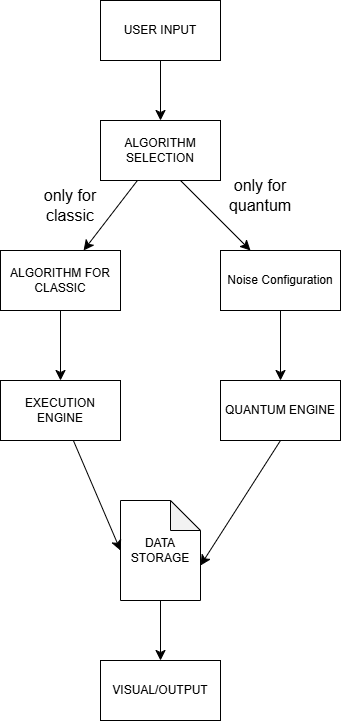
\includegraphics[scale=0.7]{proposal.png}
\caption{Rough Sketch of the Proposal Idea}
\label{fig:method}       % Give a unique label
\end{center}
\end{figure}

\begin{itemize}
\item Set up project environment and libraries. (Create Python environment, install Qiskit, NumPy, SciPy, Matplotlib, and folder structure.) - 1hr
    \item Generate optimization problem instances. (Create graphs, Max-Cut, or small TSP problems with configurable size and randomness.) - 2hr
    \item Implement simulated annealing. (Classical optimization algorithm for comparison with quantum methods, log runtime and solution quality.) -2hr
    \item Implement genetic algorithm. (Classical evolutionary approach with mutation, crossover, and selection, log metrics.) - 2hr
    \item Implement greedy/local search algorithm. (Simple heuristic for baseline performance measurement.) -2hr
    \item Implement Grover-based quantum search. (Simulate unstructured search with configurable qubits and output best solution.) - 2hr
    \item Implement QAOA quantum algorithm. (Hybrid quantum-classical variational optimization with parameter updates and solution logging.) -2hr
    \item Implement amplitude amplification. (Quantum technique for sampling and probability improvement with small problem instances.) -2hr
    \item Add noise models to quantum simulations. (Include depolarizing, dephasing, and measurement noise; allow toggling noise on/off.) - 3hr
    \item Create experiment runner. (Run multiple algorithms on multiple problem instances and collect metrics like solution quality, runtime, and stability.) - 2hr
    \item Store experiment results. (Save outputs and metadata in CSV/JSON for reproducibility and analysis.) - 1/2 hr
    \item Visualize results. (Plot solution quality, runtime, and convergence for classical vs quantum methods.) - 2hr
\end{itemize}


\bibliographystyle{acm}
\bibliography{bibliography.bib}

\end{document}
